\documentclass[compress,12pt]{beamer}
\usepackage{caption}
\usepackage{subcaption}
\usetheme{Arguelles}
\usepackage{color}
\usepackage{tcolorbox}
\usepackage{xcolor}
\usepackage{booktabs}

\newcommand{\myRed}[1]{\textcolor{red}{#1}}

\title{MATH 512 - Project 2}
\subtitle{}
\event{}
\date{}
\author{Wasif Ahmed, Haoxiang Deng, Jacob Fein-Ashley, Kanav Malhotra, Longzhe Yang}


\begin{document}

\frame[plain]{\titlepage}

\section{Question 1}

\begin{frame}{Question 1 (a)}
      We use the \emph{Kolmogorov-Smirnov} test to test for the uniformity of the random numbers generated by the LCG. The test statistic is given by
      \begin{equation*}
            D_n = \max_{1 \leq i \leq n} \left( \frac{i}{n} - U_{(i)} \right) \vee \max_{1 \leq i \leq n} \left( U_{(i)} - \frac{i-1}{n} \right)
      \end{equation*}
      where $U_{(i)}$ is the $i$-th order statistic of the $U_i$'s. 
      
      \begin{itemize}
            \item $H_{\circ}$: the random numbers are uniformly distributed. 
      \end{itemize}
      
    \begin{tcolorbox}
      We find that $D_n = 0.0069$ and a \myRed{p-value of $0.708$}. This means that we fail to reject $H_{\circ}$ at the 5\% significance level and conclude that the random numbers \myRed{are uniformly distributed.}
    \end{tcolorbox}
\end{frame}

\begin{frame}{Question 1 (a)}
      \begin{figure}
            \centering
            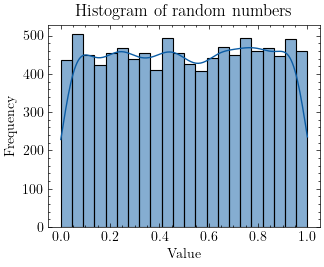
\includegraphics[scale=0.7]{imgs/1a.png}
      \end{figure}
\end{frame}

\begin{frame}{Question 1 (b)}

      Parameters: $a = 6, m = 11, x_0 = 3, c = 0,
      n=10$
      \begin{itemize}
            \item The sequence is $\{3, 7, 9, 10, 5, 8, 4, 2, 1, 6\}$
            \item The period is 10
            % \item What do you observe?
      \end{itemize}

      Parameters: $a = 6, m = 10, x_0 = 3, c = 0, 
      n=10$
      \begin{itemize}
            \item The sequence is $\{3, 8, 8, 8, 8, 8, 8, 8, 8, 8\}$
            \item The period is 1
            % \item  What do you observe?
      \end{itemize}
    \begin{tcolorbox}
    We notice that even a \emph{small} change in the parameters results in a seemingly non-random sample.
      \end{tcolorbox}
\end{frame}

\begin{frame}{Question 1 (c)}
      \begin{figure}
            \centering
            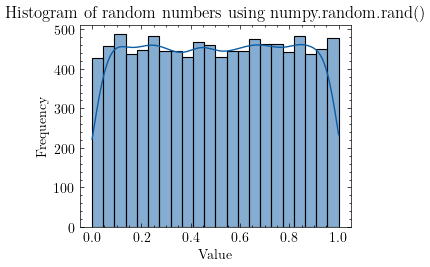
\includegraphics[scale=0.7]{imgs/1d.png}
      \end{figure}
\end{frame}

\begin{frame}{Question 1 (d)}
      \begin{figure}
            % put the histograms next to each other
            \centering
            \begin{subfigure}{0.45\textwidth}
                  \centering
                  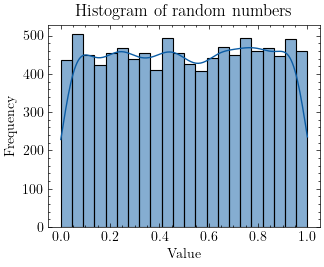
\includegraphics[scale=0.5]{imgs/1a.png}
            \end{subfigure}
            \begin{subfigure}{0.45\textwidth}
                  \centering
                  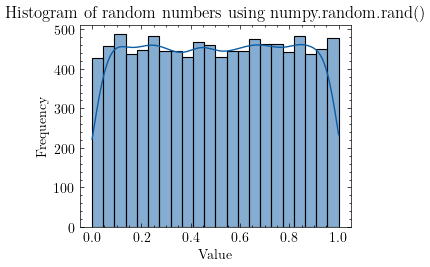
\includegraphics[scale=0.5]{imgs/1d.png}
            \end{subfigure}
      \end{figure}

      \begin{itemize}
            \item The two histograms look relatively similar, meaning both look relatively uniform.
      \end{itemize}
\end{frame}

\begin{frame}{Question 1 (e)}
      \begin{figure}
            \centering
            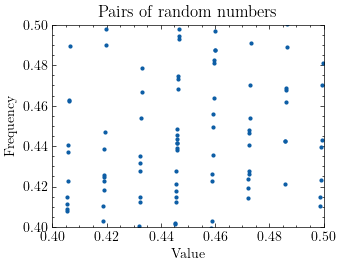
\includegraphics[scale=0.6]{imgs/pairs.png}
      \end{figure}
      \begin{itemize}
            \item The pairs of numbers seem to have a random pattern.
      \end{itemize}
\end{frame}

\begin{frame}{Question 1 (f)}
      \textbf{Disadvantages of LCG:}
      \begin{itemize}
      \begin{tcolorbox}
            \item It can appear random with the right set of parameters, but as we saw, it can get ``stuck'' in a loop.
            \item The randomness depends on the choice of parameters.
        \end{tcolorbox}
      \end{itemize}

    
\end{frame}

\section{Question 2}
\begin{frame}{Question 2}
\small{
\begin{align*}
      P(X = k) = \begin{cases}
            0.3 & \text{for } k = 1 \\
            0.2 & \text{for } k = 2 \\
            0.35 & \text{for } k = 3 \\
            0.15 & \text{for } k = 4
      \end{cases}
\end{align*}
}
We draw $10000$ random Uniform random numbers using the following rule:
\begin{align*}
      U \leq 0.3 &\implies X = 1 \\
      0.3 < U \leq 0.5 &\implies X = 2 \\
      0.5 < U \leq 0.85 &\implies X = 3 \\
      0.85 < U \leq 1 &\implies X = 4
\end{align*}     
      
\end{frame}
\begin{frame}{Question 2}
\begin{figure}
            \centering
            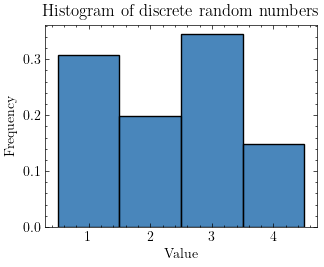
\includegraphics[scale=0.6]{imgs/discrete.png}
\end{figure}
\end{frame}

\section{Question 3}
\begin{frame}{Question 3(a) NumPy r.v. Generator}
     \begin{itemize}
         \item Observed Probability that $X < 50$: $0.00000000$.
     \end{itemize}
     \centering
     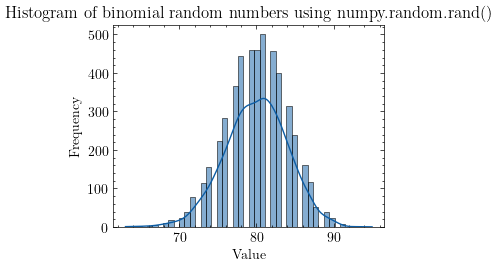
\includegraphics[scale=0.7]{imgs/binomialrv.png}
     \begin{itemize}
         \item Theoretical Probability:
     \end{itemize}
        \begin{align*}
                P(X < 50) &= \sum_{k=0}^{49} {100 \choose k} (0.8)^k (0.2)^{100-k} = {\color{red}0.00000000}
        \end{align*}
      
\end{frame}

\begin{frame}{Question 3(b) Inverse Transformation Method}
\centering
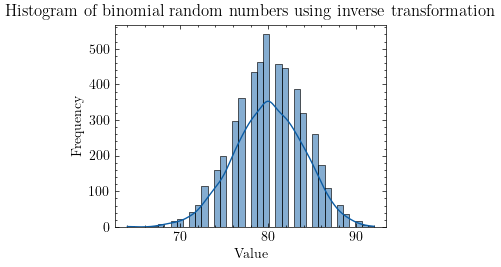
\includegraphics[scale=0.7]{imgs/binomialinverse.png}  \\
\end{frame}

\begin{frame}{Question 3(c)}
     \begin{itemize}
         \item Time for NumPy r.v. Generator: {\color{red}$0.0349$}s
         \item Time for inverse transformation method: {\color{red}$0.0350$}s
     \end{itemize} 
\end{frame}

\section{Question 4}
\begin{frame}{Question 4}
Poisson r.v. with $\lambda = 2$.
Formula:
\begin{align*}
    P(X = k) = \frac{e^{-\lambda} \lambda^k}{k!}
\end{align*}
\end{frame}
\begin{frame}{Question 4}
\centering
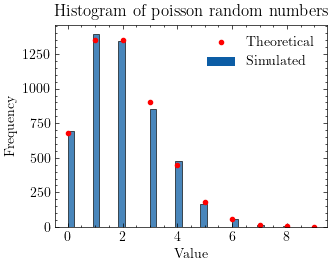
\includegraphics[scale=0.7]{imgs/poissonrv.png} 
\end{frame}

\section{Question 5}

\begin{frame}{Question 5}
      Exponential r.v. with $\lambda = 5$. \\
      Inv. Transformation Method:
      \begin{align*}
            F(x) &= 1 - e^{-\lambda x} \\
            F^{-1}(u) &= -\frac{\log(1-u)}{\lambda}
      \end{align*}

\end{frame}
\begin{frame}{Question 5}
\centering
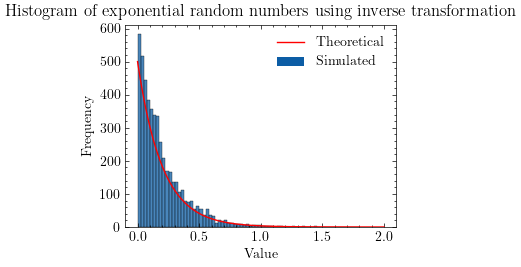
\includegraphics[scale=0.7]{imgs/exprv.png}
\end{frame}

\section{Question 6}
\begin{frame}{Question 6}
\begin{itemize}
    \item The Cauchy r.v. has the following pdf:
    \begin{align*}
        f(x) = \frac{1}{\pi(1+x^2)}
    \end{align*}
    \item We use the inverse transformation method to generate the Cauchy r.v.
    \begin{align*}
        F(x) &= \frac{1}{\pi} \arctan(x) + \frac{1}{2} \\
        F^{-1}(u) &= \tan(\pi(u - \frac{1}{2}))
    \end{align*}
\end{itemize}

\end{frame}
\begin{frame}{Question 6}
\centering
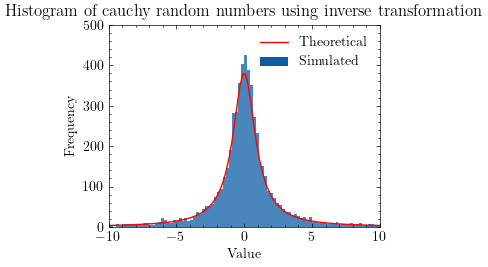
\includegraphics[scale=0.7]{imgs/cauchyrv.png}
\end{frame}

\section{Question 7}
\begin{frame}

With a repetition of $10000$ simulations, we find that {\color{red}the expectation is $1.00$} and {\color{red}the variance is $1.01$}.


We can calculate $\mathbb{E}[X]$ and $\mathbb{V}[X]$ exactly and compare them with our estimates. We have
\begin{align*}
    % expected value is 1
    \mathbb{E}[X] &= \sum_{i=1}^{100} i \cdot \frac{1}{100} = 1 \\
    % variance is 1
    \mathbb{V}[X] &= \sum_{i=1}^{100} (i - 1)^2 \cdot \frac{1}{100} - 1 = 1
\end{align*}

{\color{red}The estimates are very close to the exact values.} This is expected because the number of simulations is large.
\end{frame}

\section{Question 8: Rolling Two Die}

\begin{frame}{Question 8: Rolling Two Die}
    \textbf{Algorithm:}
    \begin{itemize}
        \item Generate two random integers in between $[1,6]$ and take the sum.
        \item Keep on generating the sum until all the integers in between $[2,12]$ are generated.
        \item Count the number of iterations it required.
        \item Repeat the same process $10000$ times.
    \end{itemize}
    \textbf{Result:} The expected number of rolls required is $\textbf{60.8352}$.
\end{frame}

\begin{frame}{Question 8: Rolling Two Dices}
\centering
\includegraphics[scale=0.2]{imgs/Rolling_Dice_HIstogram.jpg}  
\end{frame}



%\begin{frame}
%    \begin{enumerate}
%        \item Model the number of rolls needed as a geometric r.v.
%        \[
%         X \sim \text{Geometric}(p)
%         \]
%         where $p$ is the probability that all the possible outcomes have occurred at least once. 
%        \item Calculate the probability \[
%        p = \frac{6 \cdot 5 \cdot 4 \cdot 3 \cdot 2 \cdot 1}{6^6} = \frac{720}{46656} \approx 0.0154
%         \]
%        \item Calculate the expected value of $X$ as
%        \[
%        \mathbb{E}[X] = \frac{1}{p} = \frac{46656}{720} \approx 64.8
%        \]
 %        The simulation gives us an estimate of $\mathbb{E}[X] \approx 64.8$. 
 %       \item Then, the variance of $X$ is\[
 %       \mathbb{V}[X] = \frac{1 - p}{p^2} = \frac{1 - 0.0154}{0.0154^2} \approx 4151.63
%         \]
%    \end{enumerate}

%\end{frame}

\section{Question 9}
\begin{frame}{Question 9: Random Selection of 10 Balls}
    \textbf{Algorithm}
    \begin{itemize}
        \item Make an array of the following form:
$$urn=\{0,0,\cdots \text{20 times};1,1,\cdots \text{30 times};$$
$$2,2,\cdots \text{40 times};3,3,\cdots  \text{10 times}\}$$
        \item Reshuffle $urn$.
        \item Pick the first $10$ numbers and count the number of times we have $\{X_1,X_2,X_3,X_4\}=\{0,1,2,3\}.$
        \item Repeat.
    \end{itemize}
\end{frame}
\begin{frame}{Question 9: Random Selection of 10 Balls}
\centering
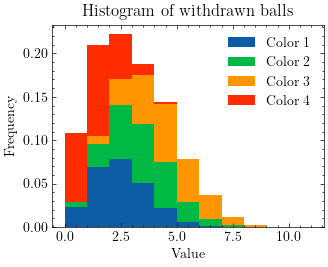
\includegraphics[scale=0.3]{imgs/balls.png}  
\end{frame}

\section{Question 10}
\begin{frame}{Question 10(a): Box-Muller Method}
    \textbf{Algorithm:}
    \begin{itemize}
        \item Generate two independent $U[0,1]$ set of random numbers: $u1$ and $u2$.
        \item Define:
        $$R=\sqrt{-2\log (u1)}$$
        $$x=\cos (2\pi u2)$$
        $$y=\sin (2\pi u2)$$
        $$z1=r*x$$
        $$z2=r*y$$
        \item Return $z1$ and $z2$.

    
    \end{itemize}
\end{frame}
\begin{frame}{Question 10 (a): Box-Muller Method}
\centering
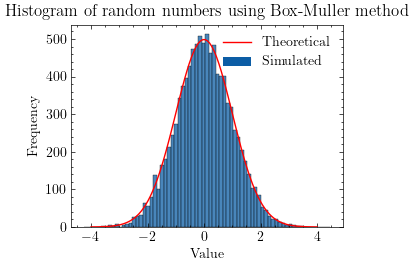
\includegraphics[scale=0.7]{imgs/boxmuller.png}  
\end{frame}

\begin{frame}{Question 10(b): Marsaglia-Bray Method}
    \textbf{Algorithm:}
    \begin{itemize}
        \item Generate two independent $U[0,1]$ set of random numbers: $u1$ and $u2$.
        \item Define:
        $$w1=(2 u1)-1$$
        $$w2=(2 u2)-1$$
        $$s=w1^2+w2^2$$
        \item if $s<1$,
        $$t=\sqrt{-2\frac{\log(s)}{s}}$$
        $$z1=w1*t$$
        $$z2=w2*t$$
        \item Return $z1$ and $z2$.
    \end{itemize}
\end{frame}

\begin{frame}{Question 10(b): Marsaglia-Bray Method}
 \centering
 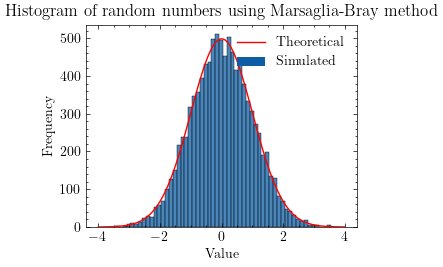
\includegraphics[scale=0.7]{imgs/marsagliabray.png}  \\
\end{frame}

\begin{frame}{Question 10(c): Acceptance-Rejection Method}
    \textbf{Algorithm:}
    \begin{itemize}
        \item Define:\\
        Normal Density Function (NDF): $\exp(\frac{-x^2}{2}/2\pi)$\\
        Proposal Density Function (PDF): $\exp(-x)$
        \item Generate $u\sim U[0,1]$ and $x\sim $PDF.
        \item $\sim 1.32 = \sqrt{2e/\pi}$
        \item if $u<\frac{\text{NDF}[x]}{1.32*\text{PDF}[x]}$, then accept $x$.
    \end{itemize}
\end{frame}

\begin{frame}{Question 10(c): Acceptance-Rejection Method}
 \centering
 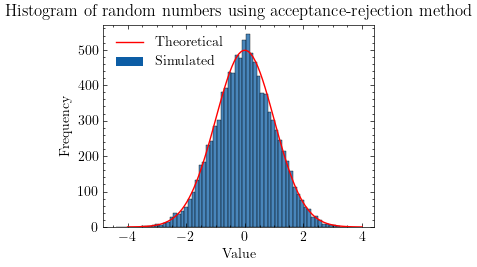
\includegraphics[scale=0.7]{imgs/acceptancerejection.png}  \\
\end{frame}


\begin{frame}{Question 10(d): $random.randn()$}
\centering
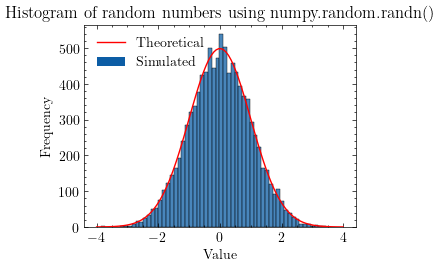
\includegraphics[scale=0.7]{imgs/numpyrandomrv.png}  \\
\begin{tcolorbox}
    All of the methods are very close to the theoretical normal distribution.  
\end{tcolorbox}

\end{frame}

\begin{frame}{Question 10: Timing}

\begin{table}[htbp]
\centering
\caption{Execution Times of Various Random Number Generation Methods}
\label{tab:execution_times}
\begin{tabular}{@{}lll@{}}
\toprule
Method & Time (ms) & Comments \\ \midrule
Box-Muller Method & 1.2269 & Fast execution \\
Marsaglia-Bray Method & 16.712 & Moderate execution \\
Acceptance-Rejection Method & 75.590 & Slow execution \\
$random.randn()$ & 0.1469 & Very fast execution \\ \bottomrule
\end{tabular}
\end{table}
    
\end{frame}



\End
\begin{frame}[plain,standout]
      \centering
      Questions?
\end{frame}

\end{document}
